\chapter{Trees}

\section{Introduction to Trees}
\begin{figure}[h!]
    \centering
    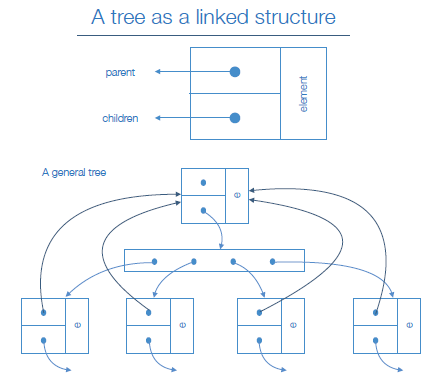
\includegraphics[width=0.75\linewidth]{immagini/general tree.png}
    \label{fig:enter-label}
\end{figure}
A \textbf{tree} is a data structure widely used to represent hierarchical relationships. It consists of nodes connected by edges and is fundamental in computer science for its structural properties. A formal tree structure satisfies the following conditions:
\begin{enumerate}
    \item It has \( n \) vertices and \( n - 1 \) edges.
    \item It is a connected graph without circuits.
    \item Any pair of vertices is connected by a unique path.
\end{enumerate}
If any of the above is true, the structure is a tree.

\section{Free Trees}
A \textbf{free tree} is a connected, acyclic, undirected graph. If a graph is acyclic but disconnected, it is termed a \textbf{forest}. Given an undirected graph \( G = (V, E) \):
\begin{itemize}
    \item If \( G \) is a free tree, any two vertices are connected by a unique path.
    \item \( G \) is connected, but if any edge is removed, the graph becomes disconnected.
    \item \( G \) has \( |E| = |V| - 1 \).
    \item \( G \) is acyclic, but adding any edge creates a cycle.
\end{itemize}

\section{Rooted Trees}
A \textbf{rooted tree} is a free tree where one of the nodes is called root.

    
\begin{figure}[h]
        \centering
        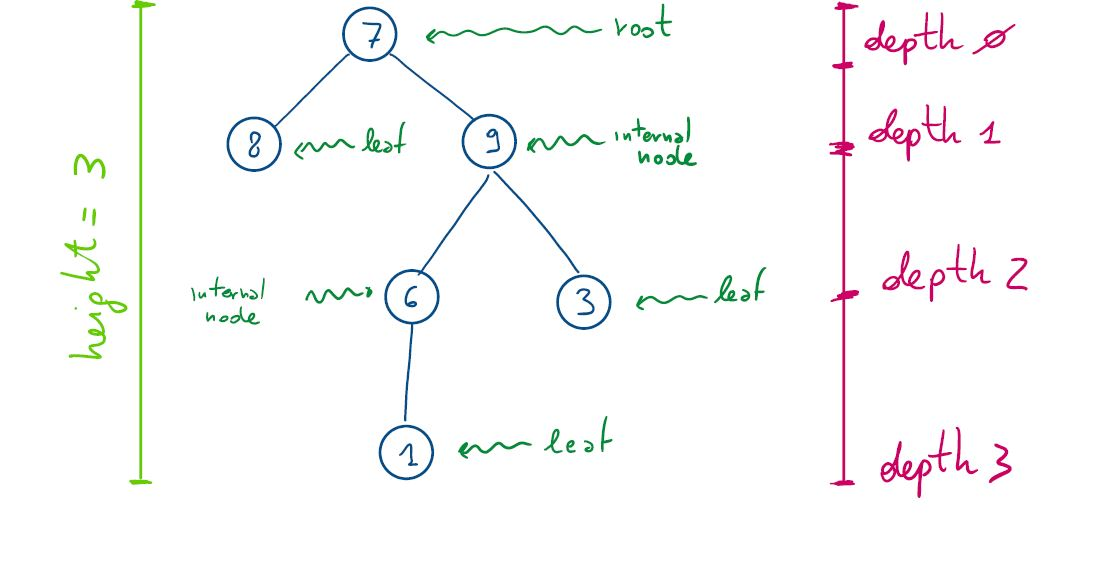
\includegraphics[width=0.5\linewidth]{immagini/rooated tree.JPG}
    \end{figure}



Each node in a rooted tree has:
\begin{itemize}
    \item \textbf{Parent}: The node directly linked above.
    \item \textbf{Child}: A node connected below.
    \item \textbf{Leaf}: A node with no children.
    \item \textbf{Internal node}: A node with at least one child.
    \item \textbf{Depth}: The level of a node from the root.
    \item \textbf{Degree}: The number of children of a node.
\end{itemize}

\subsection{Subtree and Ordered Trees}
The \textbf{subtree} rooted at \( x \) consists of \( x \) and all its descendants. In an \textbf{ordered tree}, the children of each node are arranged in a specific order (e.g.,if x has 3 children, say {y, w, z} we can say that y is the first child, w is the second child…).

\section{General Tree ADT}
The general tree Abstract Data Type (ADT) includes operations such as:
\begin{itemize}
    \item \texttt{p.element()}: Returns the element stored at position \( p \).
    \item \texttt{T.root()}: Returns the root of the tree or \texttt{None} if empty.
    \item \texttt{T.is\_root(p)}: Returns \texttt{True} if the node stored at position \( p \) is the root.
    \item \texttt{T.parent(p)}:Return the position of the parent of the node stored in \( p \).
    \item \texttt{T.num\_children(p)}: Returns the number of children of \( p \).
    \item \texttt{T.children(p)}: Generate an iteration of the children of position \( p \).
    \item \texttt{T.is\_leaf(p)} or \texttt{T.is\_external(p)}: Returns \texttt{True} if \( p \) is a leaf.
    \item \texttt{len(T)}: Returns the number of nodes.
    \item \texttt{T.is\_empty()}: Returns \texttt{True} if the tree is empty.
\end{itemize}

\section{Depth and Height of Trees}
\textbf{Depth} of a node \( p \) is the distance from \( p \) to the root. The \textbf{height} of a tree is the maximum depth among all nodes.

\subsection{Depth Calculation}
The depth of node \( p \) can be calculated using:
\begin{enumerate}
    \item Recursive method:
    \begin{verbatim}
    depth(T, p):
        if T.is_root(p):
            return 0
        else:
            return 1 + depth(T, T.parent(p))
    \end{verbatim}
    \item Iterative method:
    \begin{verbatim}
    depth(T, p):
        d = 0
        while T.parent(p) is not None:
            d += 1
            p = T.parent(p)
        return d
    \end{verbatim}
\end{enumerate}

\subsection{Height Calculation}
The height of a tree \( T \) can be computed as:
\begin{verbatim}
height(T):
    h = 0
    for each v in T.positions():
        if T.is_leaf(v):
            h = max(h, depth(T, v))
    return h
\end{verbatim}

Alternatively, using recursion:
\begin{verbatim}
height(T, p):
    if T.is_leaf(p):
        return 0
    else:
        h = 0
        for each w in T.children(p):
            h = max(h, height(T, w))
        return h + 1
\end{verbatim}

\section{Tree Traversal}
\subsection{Pre-order Traversal}
In \textbf{pre-order traversal}, the parent is visited before its children. This method is defined recursively:
\begin{verbatim}
preorder(T, p):
    visit(p)
    for each c in T.children(p):
        preorder(T, c)
\end{verbatim}
\begin{figure}[h!]
    \centering
    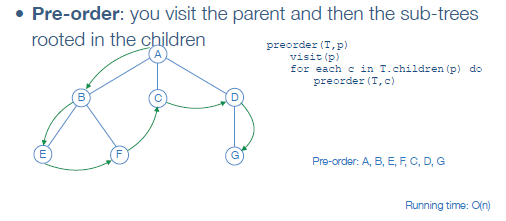
\includegraphics[width=0.75\linewidth]{immagini/tree1.png}
\end{figure}


\subsection{Post-order Traversal}
In \textbf{post-order traversal}, the children are visited before the parent.
\begin{verbatim}
postorder(T, p):
    for each c in T.children(p):
        postorder(T, c)
    visit(p)
\end{verbatim}
\begin{figure}[h!]
    \centering
    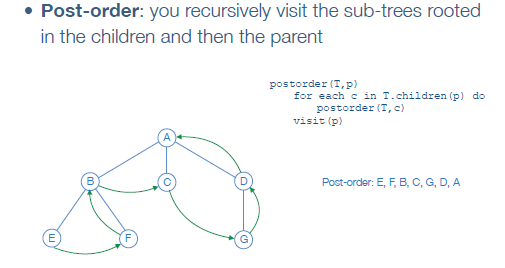
\includegraphics[width=0.75\linewidth]{immagini/tree2.png}
\end{figure}
\newpage
\subsection{Breadth-First Traversal (BFT)}
In \textbf{Breadth-First Traversal}, nodes are visited by depth level. This returns a tree. Not always it starts from left, it chooses a random child.
\begin{verbatim}
BFT(T):
    Q.enqueue(T.root())
    while not Q.is_empty():
        p = Q.dequeue()
        visit(p)
        for each c in T.children(p):
            Q.enqueue(c)
\end{verbatim}
\begin{figure}[h!]
    \centering
    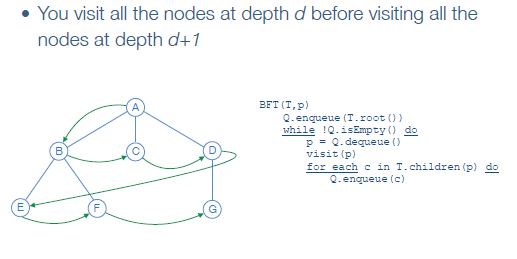
\includegraphics[width=0.75\linewidth]{immagini/tree3.png}
\end{figure}

\subsection{Exercise}
\begin{figure}[h!]
    \centering
    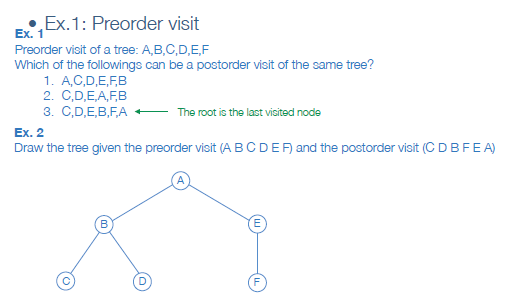
\includegraphics[width=1\linewidth]{immagini/tree4.png}
\end{figure}

\section{Binary Trees and Binary Search Trees (BST)}
A \textbf{binary tree} has each node with at most two children (left and right), the left child comes before the right child in the order of children of a node.
A binary tree is called \textbf{proper(or full)} if every node has zero or two children.
\begin{figure}[h!]
    \centering
    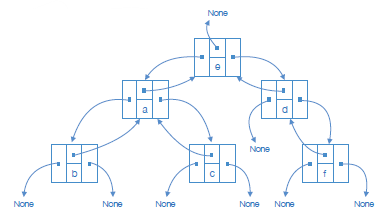
\includegraphics[width=0.75\linewidth]{immagini/tree5.png}
\end{figure}
A \textbf{Binary Search Tree (BST)} is an ordered binary tree where:
\begin{itemize}
    \item For any node \( x \), nodes in the left subtree of \( x \) have keys \( \leq x \).
    \item Nodes in the right subtree have keys \( \geq x \).
\end{itemize}
In other words: is a rooted binary tree data structure whose internal nodes each store a key greater than all the keys in
the node’s left subtree and less than those in its right subtree.

\paragraph{Complete and Full Binary Trees} There are many types of binary trees, but we will focus on two: complete and full.
\begin{itemize}
    \item \textbf{Full binary tree}: Every node has either 0 or 2 children.
    \item \textbf{Complete binary tree}: Every node has either 0 or 2 children, except for the last level, which may have some missing nodes. These nodes must be filled from left to right. A complete binary tree is also a heap.
\end{itemize}


\subsection{Binary Tree Traversal: In-Order}
In-order traversal for BST visits nodes from left to right:
\begin{verbatim}
inorder(T, x):
    if x is not None:
        inorder(T, x.left)
        visit(x)
        inorder(T, x.right)
\end{verbatim}
\begin{figure}[h!]
    \centering
    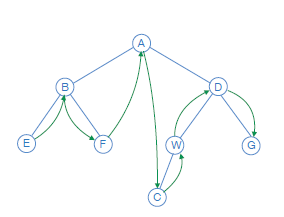
\includegraphics[width=0.6\linewidth]{immagini/tree6.png}
\end{figure}
\section{BST Operations}
Key operations in a BST include:
\begin{itemize}
    \item \textbf{Search}: Finding a node with a given key.
    \item \textbf{Minimum and Maximum}: Finding the smallest or largest element. By keeping going down to the left you will find the minimum, by going to the right you will find the maximum.
    \item \textbf{Successor and Predecessor}: Finding the next or previous node in sorted order.
\end{itemize}
\subsection{Binary Search Example: Tree-Search}
Searching for a key \( k \) in a BST starting from root node \( x \). Inputs: x is a given node where the search starts (usually the root) and k is the key to be searched in the tree. Outputs: a pointer to a node with key k or NIL if the key is not in the tree.

\begin{verbatim}
TREE-SEARCH(x, k):
    if x == NIL or k == x.key:
        return x
    if k < x.key:
        return TREE-SEARCH(x.left, k)
    else:
        return TREE-SEARCH(x.right, k)

ITERATIVE-TREE-SEARCH(x,k):
    while x!=NIL and k!=x.key() do
        if k<x.key
            x = x.left
        else
            x = x.right
    return x
\end{verbatim}

\begin{figure}[h!]
    \centering
    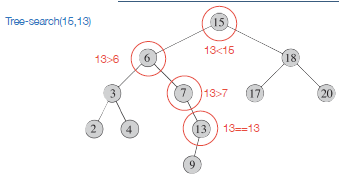
\includegraphics[width=0.75\linewidth]{immagini/tree7.png}
\end{figure}
The nodes encountered during the process form a path downward from the root, thus we visit a number of nodes which equals the height of the node k in the tree. Complexity: O(h) where h is the height
\newpage Exercise: Suppose we have numbers between 1 and 1000 in a binary search tree, and we want to search for the number 364. Which of the following sequences cannot be the sequence of nodes examined?
\begin{itemize}
    \item 1,252,401,398,330,344,397,364
    \item 924,220,911,244,898,258,362,364
    \item 925,202,911,240,912,245,364
\end{itemize}
There answer is the third option since 912 cannot belong to the left subtree of 911.

\subsection{Successor: Property}
Given a binary search tree \( T \) and \(x, y \) in \( T \) 
Given a binary search tree T and x,y in T, then \( y \) is a successor of \( x \) if \( y.key>x.key \) and there not exist a
 \( z \) in \( T \) such that \(  y.key> z.key >x.key\).  $\\$
 
\textbf{Property:} Consider a binary search tree T whose keys are distinct. If the right subtree of a node \(x\) in \(T\) is empty and \(x\) has a successor \(y\), then \(y\) is the lowest ancestor of \(x\) whose left child is also an ancestor-orself
of \(x\).
Note: in this case we consider a node to be an ancestor of itself.
The running time is O(h) since we either follow a simple path downwards or a simple path upwards.
\begin{figure}[h!]
    \centering
    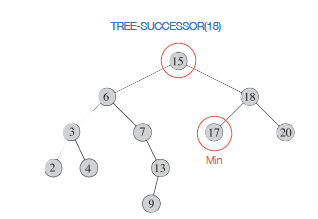
\includegraphics[width=0.75\linewidth]{immagini/tree8.png}
\end{figure}

    


